\documentclass[10pt, conference, letterpaper]{IEEEtran}
\usepackage{cite}
\usepackage{xcolor,soul,framed}
\usepackage{amsmath,amssymb,amsfonts}
\usepackage{algorithmic}
\usepackage{graphicx}
\graphicspath{ {./images/} }

\begin{document}

    %=============================== TITLE ===============================%
    \title{
        Delay Optimal Dispatching with Obsolete Broadcast Two-Time Scale MDP
    }
    \author{
        \IEEEauthorblockN{HONG Yuncong}
        \IEEEauthorblockA{
            \textit{Department of CS}, The University of Hong Kong, China \\
            ychong@cs.hku.hk
        }
    }
    \maketitle

    %============================== ABSTRACT ==============================%
    \begin{abstract}
        \label{sec:abstract}
        We formulate the problem with job dispatching in distributed Edge Computing system, and we identify the difficulty exists in delayed cooperation between different APs (Access Points) and ESs (Edge Servers) to 
        \\
        (in progress)
    \end{abstract}

    \begin{IEEEkeywords}
        Edge Computing, Delayed Information, Two-time Scale MDP
    \end{IEEEkeywords}

    %============================ INTRODUCTION ============================%
    \begin{section}{INTRODUCTION}
        \label{sec:introduction}
        (in progress)
        \cite{sutton1998introduction}
    \end{section}

    %========================= LITERATURE REVIEW ==========================%
    % \begin{section}{LITERATURE REVIEW}
    %     \label{sec:review}
    % \end{section}

    %============================ FORMULATION =============================%
    \begin{section}{FORMULATION}
        \label{sec:formulation}
        In this section, we will firstly give the definition of the proposed problems. Then we will give the insight of problem solving with the global optimization problem, and why some states are not attainable in the local version. At last, we show that with the broadcast design we could solve the original problem with a larger time scale sub-optimization, which is called a two-time-scale MDP problem.

        \begin{subsection}{Problem Definition}
            In a Mobile Edge Computing system, jobs arrive at each AP, and the decision is made on AP to dispatch to the Edge servers. Then the scheduling policy is carried out on each server to facilitate the global optimization target (which is heuristic).
            \\
            Computation model: unrelated parallel machine, with prioritized task on independent server

            \begin{subsubsection}{Communication Model}
                The communication model in our system ignores the underlaid real communication channel underlaid, instead of simple probabilistic distribution.
                The communication time between each AP and ES is: fixed uploading time, and fixed broadcast delay;
                For now, we don't take the broadcast cost into consideration because it's not easily evaluated in the complicated network model (without specified).
            \end{subsubsection}

            \begin{subsubsection}{Deterministic Computation Model}
                The computation happened on each ES is deterministic, and the computation time of each job is known previously when arrival at APs.
            \end{subsubsection}

            \begin{subsubsection}{Optimization Target}
                (to minimize the average job response time)
            \end{subsubsection}

            So, we hope to apply the policy at AP side and then establish
        \end{subsection}

        \begin{subsection}{Global MDP Problem}
            In this section, we give out he definition of the previous problem under the framework of MDP.

            \begin{subsubsection}{Markovian States}
                We take the problem description at the grain of jobs and we choose job set as our states (given that broadcast delay is fixed, the length vector of fractions would be also fixed).
            \end{subsubsection}

            \begin{subsubsection}{Update Rules and Transition Function}
                \begin{figure}[h]
                    \label{fig:trans}
                    \centering
                    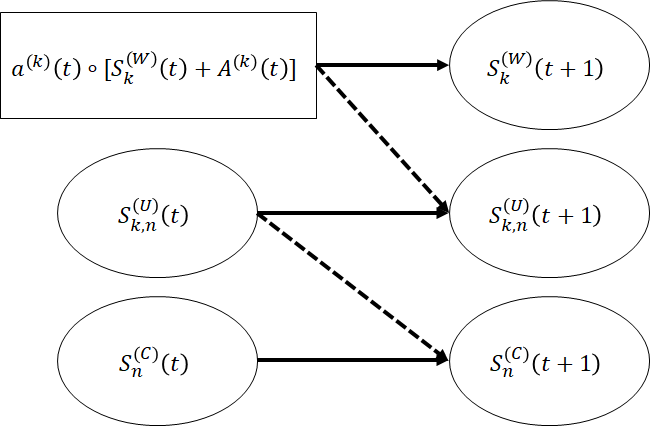
\includegraphics[width=0.45\textwidth]{single-transition.png}
                    \caption{Single-step transition function composing illustration}
                \end{figure}
            \end{subsubsection}

            \begin{subsubsection}{Cost Function and Bellman Equation}
                (Value function in Bellman equation format, and average cost function brought by transition function)
                As we are considering broadcast delay, we could re-consider the broadcast information as partially observed collected information lasting for $\hat{x}_k$ time slots.
                \\
                However, according to our previous assumption: the communication delay according to propagation delay is also comparable to arrival interval and is not negligible; but we could have \emph{piggyback} to make it work.
            \end{subsubsection}
        \end{subsection}

        \begin{subsection}{Local MDP Problem}
            We formulate the local MDP optimization problem, with the same target as global value function. As the policy applied on each AP could not obtain the global information, we design the broadcast for every nodes to share their local states to other nodes (APs).
            
            However, due to the broadcast delay, we could not optimize the original global optimization problem based on states on one single AP. So we develop the local MDP problem with collected broadcast information.

            \begin{subsubsection}{Broadcast Denotations}
                The illustration figure \ref{fig:brd} for single broadcast includes several important time points which are also important in multiple asynchronous broadcast: $x_{k,*}, d_{k,*}, T^{br}_{k,*}$

                \begin{figure}[h]
                    \label{fig:brd}
                    \centering
                    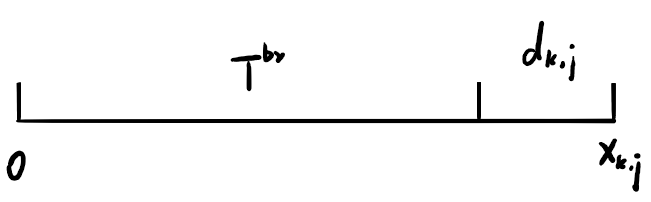
\includegraphics[width=0.45\textwidth]{single-broadcast.png}
                    \caption{Single broadcast timing illustration}
                \end{figure}

                And with the implication from the single broadcast, we generalize the conclusion for every broadcasts with:
                $$
                x_{k,*} = d_{k,*} + T^{Br}_{*}
                $$
                which takes a reasonable assumption that $T>d$ always ($*=k'$ or $n$ for $k$-th AP).

                Then we come up with the idea with collected broadcast states, which are splitted by the maximum broadcast interval which is denoted as $\hat{x}_k$:
                $$
                \hat{x}_k = \max(x_{k,*})
                $$
                And we denote all the partial or completed observed information (states of other nodes) in this smallest covering interval as $\Delta$.
                We notice that there is one periodic behavior as the broadcast interval is fixed for each node, and the period is simply obtained by LCM (Least Common Multiple):
                \begin{align*}
                    p_{k} &= \bar{x}_k/\hat{x}_k
                    \\
                    \bar{x}_k &= lcm(x_{k,*})
                \end{align*}
                And the series of states over time is denoted as:
                $$
                \{ \Delta^{(k)}_1 \to \dots \to \Delta^{(k)}_{p_k} \} \to \Delta_{1}
                $$
                
                The periodic behavior with the total $p_k$ behavior could be explained with \textit{information gap} in each period as $r_{k,*}$. Here we allows the time slot to be counted with $Z_+$, then we define the broadcast interval as \textit{additive modulo group} with respect to each node to $k$-th AP as $Z_{x_{k,*}}$.
                \begin{align}
                    & \hat{d}_{k,*}^{(i)} \equiv i \times \hat{x}_k \pmod{x_{k,*}}
                    \\
                    \text{and } & r_{k,*} \equiv \hat{x}_k \pmod{x_{k,*}}
                    \\
                    \text{so: } & \hat{d}_{k,*}^{(i)} = i \times r_{k,*}
                \end{align}
            \end{subsubsection}

            \begin{subsubsection}{Multi-step Update Rule}
                the multi-step transition is not simply iteratively run the single-step transition. Because the transition is confined by information from other nodes, the probability distribution would be deducted with Bayes' Law.

                Here we develope the rule for multi-step update.
            \end{subsubsection}

            \begin{subsubsection}{Total Transition and Bellman Equation}
                The total transition function could be obtained via the previous update rules, which we denote as $T(\Delta_{i-1}, a_{\Delta_{i-1}}, \Delta_{i})$
            \end{subsubsection}

            \begin{subsubsection}{Optimality Gap to Global Optimization}
                (in progress)
            \end{subsubsection}
        \end{subsection}

    \end{section}

    %============================= ALGORITHM ==============================%
    \begin{section}{ALGORITHM}
        \label{sec:algorithm}
        (in progress)
    \end{section}

    %============================ EVALUATION ==============================%
    \begin{section}{EVALUATION}
        \label{sec:ealuation}
        (in progress)
    \end{section}

    %============================= CONCLUSION =============================%
    \begin{section}{CONCLUTION}
        \label{sec:conclusion}
        (in progress)
    \end{section}

    %============================== REFERENCE =============================%
    \bibliographystyle{IEEEtran}
    \bibliography{main.bib}
\end{document}